\chapter{Uniwersalna architektura procesorów wielordzeniowych}
Rozdział ten stanowi wprowadzenie to zagadnienia obliczeń wielordzeniowych. Przedstawiona została w nim pokrótce historia rozwoju oprogramowania oraz sprzętu komputerowego, który podążał za co raz to wyższymi wymaganiami stawianymi przez użytkowników. Opisana zostanie również historia rozwoju \emph{procesora} (\acronym{CPU}, \english{Central Processing Unit}) - głównej jednostki obliczeniowej w praktycznie każdym urządzeniu elektronicznym. Później opisany zostanie rozwój karty graficznej oraz zmiana jej zastosowania na przestrzeni lat. 

Ostatnim, lecz nie najmniej ważnym elementem tego rozdziału jest opis uniwersalnej architektury obliczeniowej CUDA (\english{Compute Unified Device Architecture}) wprowadzonej przez firmę nVidia w roku 2007, która umożliwia wykorzystanie mocy obliczeniowej \termdef{procesorów graficznych} (\acronym{GPU}, \english{Graphics Processing Unit}), bądź innych procesorów wielordzeniowych, do rozwiązywania ogólnych problemów obliczeniowych w sposób znacząco wydajniejszy niż w przypadku tradycyjnych, sekwencyjnych procesorów~\cite{cuda:zone}.

Na rysunku~\ref{rys:gpu_cpu} przedstawiony został przyrost w przepustowościach pamięci - odpowiednio dla GPU oraz CPU na przestrzeni lat. Łatwo zauważyć, że w ciągu 7 lat procesor graficzny zyskał około 10-krotną przewagę nad CPU. Dlatego też co raz większe jest zainteresowanie wykorzystaniem kart graficznych w dziedzinach innych niż tylko renderowanie grafiki.

\begin{figure}[h]
\centering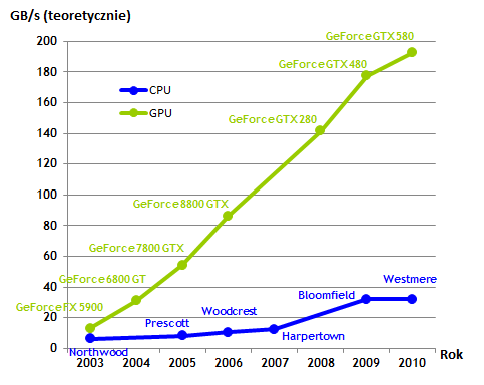
\includegraphics[width=0.9\textwidth]{figures/03/gpu_cpu.png}
\caption{Przepustowość pamięci na CPU oraz GPU~\cite{Cuda:PGuide}}\label{rys:gpu_cpu}
\end{figure}

\section{Czasy przetwarzania równoległego}
W poprzednich latach dokonał się znaczący postęp w przechodzeniu przemysłu komputerowego na obliczenia wykonywane równolegle. W roku 2010 większość komputerów konsumenckich była dostarczana do odbiorcy z procesorem zawierającym więcej niż jeden \emph{rdzeń} (\english{core}). Począwszy od procesorów dwurdzeniowych w laptopach do 8- czy 16-rdzeniowych stacji roboczych - od pewnego czasu obliczenia równoległe nie są już tylko domeną superkomputerów lub mainframe'ów (ang. \emph{main} – główny, \emph{frame} – struktura). Co więcej, urządzenia elektroniczne takie jak telefony komórkowe czy też przenośne odtwarzacze muzyki wyposażane są w procesory wielordzeniowe, co zapewnia im możliwości dalece przekraczające te dostępne dla ich poprzedników.

Wynika z tego, że coraz to więcej programistów będzie musiało radzić sobie z implementacją oprogramowania przeznaczonego na jednostki równoległe, wykorzystywać nowe technologie, które będę pozwalały na dostarczenie nowatorskich rozwiązań dla co raz bardziej wymagającej rzeszy użytkowników. Wiersze poleceń to przeżytek - od dawna komputerem steruje się za pomocą skomplikowanych interfejsów graficznych. To samo tyczy się telefonów komórkowych - w chwili obecnej telefon to tylko jedna z wielu funkcji, jakich może dostarczyć współczesny aparat telefoniczny. Teraz telefony mogą jednocześnie grać muzykę, dostarczać informacji o obecnej lokalizacji przy użyciu modułu nawigacji satelitarnej (\acronym{GPS}, \english{Global Positioning System}) i jednocześnie wyświetlać zdjęcia.

\subsection{Procesor}\label{03-procesor}
Przez około 30 lat jedną z ważniejszych metod udoskonalania centralnych jednostek obliczeniowych, a przez to zwiększania komfortu korzystania z urządzenia przez użytkownika, było zwiększanie prędkości z jaką operował zegar procesora. W latach 80 XX wieku procesor przeznaczony na rynek konsumencki operował z prędkością oscylującą w okolicach $1$MHz. Około 30 lat później, w czasach współczesnych, większość komputerów osobistych wyposażona jest w procesory o prędkościach od $1$ do $4$GHz, czyli obecne jednostki są około $1000$ szybsze od wczesnych procesorów. Zwiększanie prędkości, z jaką operuje zegar procesora jest niezawodnym źródłem zwiększania szybkości, należy jednak podkreślić, że nie jest to jedyna metoda na zwiększanie jego wydajności.

Jednakże ograniczenia technologiczne wyznaczają pewne granice, w jakich może wzrastać prędkość zegara procesora. Dlatego też poszukuje się innych, równie niezawodnych źródeł zwiększenia wydajności. Nie można już dłużej polegać jedynie na zwiększaniu prędkości. Z powodu restrykcji na mocy oraz wydzielanym cieple oraz docieraniu do granicy rozmiaru tranzystora, naukowcy oraz producenci rozpoczęli poszukiwanie nowych źródeł i sposobów na zwiększenie możliwości procesorów.

Poza światem konsumentów, czyli w świecie tzw. superkomputerów przez dekady osiągano niezwykle wielkie przyrosty mocy w bardzo podobny sposób. Moc procesora używanego w tych komputerach rosła tak samo szybko, jak w przypadku przyrostów procesorów desktopowych. Jednakże, poza wielkimi przyrostami mocy obliczeniowej na jednej jednostce, producenci superkomputerów tworzyli komputery, w których solidne przyrosty w wydajności osiągano dzięki zwiększaniu liczby używanych procesorów. Nie jest niczym niezwykłym, że pojedynczy superkomputer składa się z dziesiątek lub setek tysięcy procesorów działających równolegle.

W poszukiwaniu dodatkowych możliwości dla komputerów osobistych, poprawa wydajności w przypadku superkomputerów rodzi pytanie: Dlaczego zamiast zwiększać wydajność pojedynczej jednostki, nie umieścić w komputerze osobistym więcej rdzeni? W wypadku zwiększania liczby rdzeni rozwój jednostek obliczeniowych nie byłby ograniczony przez te same niedogodności, co w przypadku ciągłego zwiększania prędkości zegara procesora.

W roku 2005 wiodący producenci prosesorów zaczęli oferować jednostki z dwoma, zamiast z jednym rdzeniem. W latach następnych kontynuowano tę praktykę, tworząc jednostki trzy-, cztero-, sześcio- oraz ośmio-rdzeniowe. Czasami nazywa się ten okres \emph{rewolucją wielordzeniową}~\cite{Cuda:Example}, ponieważ zmiana podejścia do zwiększania wydajności jednostek w znaczący sposób wpłynęła na ewolucję konsumenckiego rynku komputerów.

W chwili obecnej praktycznie każdy komputer osobisty jest wyposażony w procesor dwurdzeniowy. Nawet na rynku niskobudżetowych komputerów z bardzo niskim zapotrzebowaniem na moc, dokonała się rewolucja wielordzeniowa - już nawet netbooki będą wyposażone w dwa rdzenie~\cite{intel:netbook}. 

\section{Wpływ procesorów graficznych na procesy obliczeniowe}

Wydawać by się mogło, że użycie procesora graficznego, jako jednostki obliczeniowej dla problemów nie związanych bezpośrednio z przetwarzaniem grafiki jest podejściem zupełnie nowym. Porównując to do klasycznych obliczeń na procesorach jest to w istocie konepcja nowa. Jednakże obliczenia na jednostkach graficznych nie są tak nowe, jak mogłoby się wydawać na pierwszy rzut oka. 

\subsection{Krótka historia kart graficznych}

W rozdziale~\ref{03-procesor} przedstawiony został rozwój procesora w dwóch płaszczyznach - prędkości oraz liczbie rdzeni. W międzyczasie karty graficzne przeżywały rewolucję rozwojową. Na końcu lat 80 oraz początku 90, wzrost popularności \emph{graficznych interfejsów użytkownika} (\acronym{GUI}, \english{Graphical User Interface}), a w szczególności systemów operacyjnych takich jak Microsoft Windows, wymusił na producentach sprzętu stworzenie nowego typu procesora. We wczesnych latach 90 użytkownicy zaczęli kupować karty graficzne 2D dla swoich komputerów osobistych. Te akceleratory grafiki oferowały wsparcie sprzętowe do operacji bitmapowych by umożliwić wykorzystanie graficznego interfejsu użytkownika.

Mniej więcej w tym samym czasie, w świecie profesjonalnych komputerów, firma o nazwie \emph{Silicon Graphics} popularyzowała w latach 80-tych użycie grafiki trójwymiarowej w wielu dziedzinach, m.in. aplikacje rządowe oraz obronne, aplikacje wspierające naukę oraz wizualizację wyników przeprowadzanych badań naukowych, a także w tworzeniu trójwymiarowych efektów filmowych, czyli rzeczy do tej pory niedostępnych na rynku. W roku 1992 Silicon Graphics stworzyło interfejs programistyczny do swojego sprzętu poprzez wydanie biblioteki IRIS GL, która następnie wyewoluowała do OpenGL (\english{Open Graphics Library}), czyli specyfikacji uniwersalnego API do generowania grafiki. Firma ta wypuszczając tę bibliotekę chciała, by była ona ustandaryzowaną, niezależną od platformy biblioteką do tworzenia aplikacji trójwymiarowych. Zupełnie, jak w pryzpadku licznych rdzeni na procesorach (patrz rozdział~\ref{03-procesor}) było tylko kwestią czasu, aż aplikacje 3D znajdą się w domach użytkowników na ich prywatnych komputerach.

\begin{figure}[h]
\centering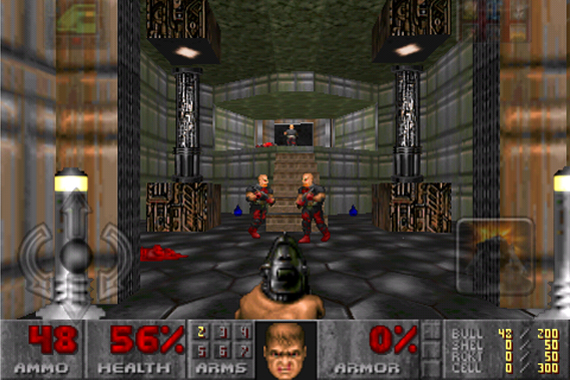
\includegraphics[width=0.9\textwidth]{figures/03/doom.png}
\caption{Zrzut ekranu z gry DOOM - klasycznej gry z gatunku FPS}\label{rys:doom}
\end{figure}

Dwa znaczące powody w połowie lat 90-tych spowodowały, że pojawiła się nagła potrzeba stworzenia procesora graficznego potrafiącego tworzyć trójwymiarowe efekty (\acronym{3D}, \english{three-dimensional}). Pierwszym było pojawienie się wciągających gier, w których gracz ogląda świat gry z perspektywy pierwszej osoby, czyli oczami bohatera (\acronym{FPP}, \english{First Person Perspective}), takich jak Doom (patrz rysunek~\ref{rys:doom}), Duke Nukem 3D oraz Quake. Przyczyniło się to do rozpoczęcia tworzenia bardziej realistycznych środowisk trójwymiarowych, w których możliwe byłoby tworzenie gier komputerowych. Pomimo tego, że grafika 3D mogła być wykorzystana w praktycznie wszystkich grach komputerowych, to wyjątkowa popularność gier z gatunku FPS (\english{First Person Shooter}) spowodowała, że większy nacisk położono na prywatne jednostki komputerowe. W tym samym czasie firmy takie jak NVIDIA, ATI Technologies oraz 3dfx Interactive zaczęły produkować akceleratory graficzne, które były w stanie sprostać ciągle rosnącym wymaganiom klientów. Te strategiczne decyzje spowodowały, że grafika trójwymiarowa na dobre zadomowiła się na komputerach stacjonarnych i w nadchodzących latach to ona miała wieść prym wśród technologii komputerowych.

\begin{figure}[h]
\centering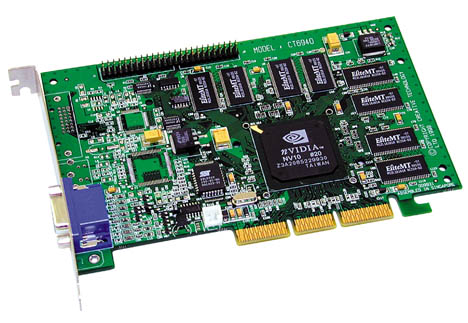
\includegraphics[width=0.7\textwidth]{figures/03/geforce-256.jpg}
\caption{Karta graficzna NVIDIA GeForce 256}\label{rys:gf256}
\end{figure}

Wypuszczenie w drugiej połowie roku 1999 na rynek karty graficznej NVIDIA GeForce 256 przesunęło możliwości komputerów osobistych jeszcze dalej~\cite{nvidia:geforce256} - wygląd tej karty przedstawiony został na rysunku~\ref{rys:gf256}. Po raz pierwszy obliczenia świetlne oraz transformacje obliczeniowe możliwe były do wykonania bezpośrednio na procesorze graficznym, co dawało jeszcze większe możliwości tworzenia aplikacji atrakcyjnych wizualnie. Ponieważ operacje te były już integralną częścią \emph{potoku wywołań} (\english{pipeline}) biblioteki OpenGL, karta GeForce 256 wyznaczyła początek progresywnego zwiększania operacji dostępnych w biliotece OpenGL, które były implementowane na procesorze graficznym.

Uważa się, że wypuszczona w roku 2001 seria kart graficznych GeForce 3 jest jednym z większych przełomów w świecie technologii GPU~\cite{nvidia:geforce3,Cuda:Example}. Seria ta była pierwszą w świecie, której chip był kompatybilny z nowym w ówczesnym czasie standardem firmy Microsoft o nazwie DirextX 8.0, który wymagał by hardware zawierało \emph{programowalne wierzchołki} (\english{programmable vertex}) oraz \emph{programowalne cieniowanie} (\english{programmable pixel shading}) w kolejnych fazach przetwarzania. Po raz pierwszy programiści mogli mieć jakąkolwiek kontrolę nad obliczeniami dokonywanymi bezpośrednio na karcie graficznej.

\subsection{Wczesne obliczenia na kartach graficznych}
\label{chapter:wczesne}

Wyprodukowanie kart, które posiadały następujące po sobie programowalne fazy (potok wywołań) spowodowały, że wielu naukowców zaczęło wykorzystywać ich możliwości nie tylko poprzez używanie OpenGL czy też DirectX do standardowych zadań. Takie podejście do obliczeń na kartach graficznych we wczesnych latach obliczeń na GPU było niezwykle skomplikowane. Ponieważ standardowe API graficzne takie jak OpenGL, czy też DirectX były jedynymi metodami do interakcji z GPU, to programowanie obliczeń na kartach graficznych nadal sprowadzało się do implementowania przetwarzania graficznego poprzez dotępne metody interfejsu programistycznego karty. Z tego też powodu, wielu naukowców wykonywało swoje obliczenia poprzez wspomniane wcześniej API w taki sposób, by ich problemy sprowadzone zostały do renderowania grafiki, a następnie odpowiedniego przetworzenia.

Zasadniczo każda karta graficzna we wczesnym roku 2000 zaprojektowana była w taki sposób, by produkować kolor dla każdego piksela na ekranie używając programowalnych jednostek arytmetycznych nazywanych \emph{pixel shader}. W ogólności jednostka ta wykorzystuje pozycję (jako parę $(x, y)$) piksela oraz pewne dodatkowe informacje by obliczyć kolor danego piksela na ekranie. Tymi dodatkowymi informacjami mogą być kolory, wymiary tekstur oraz parametry, które mogą zostać podane, bądź obliczone w trakcie interakcji z użytkownikiem, bądź otoczeniem piksela. Ponieważ obliczenia wykonywane na wejściowych kolorach oraz teksturach były kontrolowane przez programistę, zauważono, że te wejściowe ,,kolory'' mogą w rzeczywistości reprezentować dowolną daną.

Zatem jeśli wejście programu było dowolną daną reprezentowaną jako wartość reprezentującą coś zupełnie innego niż wartość, to programiści mieli możliwość wykorzystywania pixel shaderów, czyli krótkiego programu komputerowego w specjalnym języku, do wykonania na tych danych porządanych obliczeń oraz przekształceń. Rezultatem tych obliczeń był ,,kolor'', który w danym kontekscie oznaczał coś zupełnie innego niż tylko kolor na ekranie w dosłownym tego słowa znaczeniu. Można więc nazwać to ,,oszukiwaniem'' karty graficznej poprzez poddawanie danych wejściowych przetwarzaniu graficznemu, jakby były to zwyczajne dane potrzebne do wyrenderowania obrazu. Takie podejście odznaczało się wyjątkowym poziomem pomysłowości, ale niestety wykonanie takich obliczeń było wyjątkowo zagmatwane i skomplikowane.

Z powodu wysokiej przepustowości obliczeń arytmetycznych na GPU, początkowe rezultaty takich eksperymentów obiecywały świetlaną przyszłość obliczeń na jednostkach graficznych. Jednakże model programistyczny stosowany do implementacji takich obliczeń był zbyt restrykcyjny dla rzeszy developerów by mógł być wykorzystywany na szeroką skalę. Możliwe było jedynie wykorzysytwanie ,,kolorów'' oraz podmian tekstur, co w wielu przypadkach stanowiło duże ograniczenie przy bardziej skomplikowanych obliczeniach. Było również sporo ograniczeń do do tego jak i gdzie programista mógł zapisywać wyniki do pamięci karty, tak więc algorytmy wykorzystujące rozproszone lokacje nie były możliwe do implementacji na GPU. Co więcej, bardzo trudno było implementować algorytmy korzystające z obliczeń zmiennopozycyjnych (\english{floating-point}), ponieważ nie można było przewidzieć, jak karta graficzna, jeśli w ogóle, wykona te obliczenia~\cite{Cuda:Example}. Ostatnim z zasadniczych ograniczeń był fakt braku jakiejkolwiek metody do debugowania kodu uruchamianego na karcie graficznej - na przykład w momencie wyraźnie błędnych obliczeń, zawieszania się komputera czy też w momencie nie zakończenia się programu.

Jeśli wcześniej wymienione ograniczenia nie były przeszkodą, ktokolwieek kto chciał wykorzystać moc obliczeniową karty raficznej do wykonywania obliczeń nie związanych z przetwarzaniem grafiki musiał w dalszym ciągu nauczyć się OpenGL bądź DirectX, gdyż to one pozostawały jedynymi metodami do interakcji z GPU. Nie tylko oznaczało to przechowywanie wyników w teksturach graficznych oraz wykonywania obliczeń poprzez wywoływanie funkcji OpenGL lub DirectX, ale dodatkowo oznaczało to pisanie obliczeń w specjalnych językach programowania graficznego (\english{shading languages}). Wymaganie by naukowcy dokonywali obliczeń na ograniczonych zasobach oraz specjalnych językach programowania oraz nauczenia się specyfiki jednostek graficznych przed przystąpieniem do wykorzystania możliwości GPU do obliczeń spowodowało, że metoda ta nie przyjęła się, jako wiodąca w świecie naukowców.

\section{CUDA}

Dopiero po około pięciu latach od wydania serii 3 GeForce obliczenia na jednostkach graficznych były gotowe rzeczywiście być implementowane przez programistów z pełnym wykorzystaniem możliwośći kart. W listopadzie 2006 roku NVIDIA wypuściła na rynek pierwszą kartę graficzną wspierającą DirectX 10 - GeForce 8800 GTX~\cite{nvidia:geforce8800}. Karta ta była również pierwszą jednostką zbudowaną na architekturze CUDA. Architektura ta zawierałą nowe komponenty zaprojektowane specjalnie pod obliczenia wykonywane na GPU oraz eliminowała wiele ograniczeń, które powstrzymywały programistów przed wykorzystywaniem możliwości karty do obliczeń nie związanych z przetwarzaniem grafiki.

\subsection{Czym jest architektura CUDA?}

W przeciwieństwie do poprzednich generacji kart graficznych, w których jednostki były podzielone na pixel i vertex shader'y, w kartach zgodnych z architektura CUDA zawarta jest zunifikowana linia shaderów (\english{shader pipeline}). Pozwala to każdej jednostce arytmetyczno-logicznej (\acronym{ALU}, \english{Arithmetic Logic Unit} lub \emph{Arithmetic and Logical Unit}) na czipie być wykorzystaną przez program wykonujący podstawowe operacje obliczeniowe.

Ponieważ firma NVIDIA zamierzała tę nową rodzinę kart graficznych była wykorzystywana w innych rejonach niż tylko wyświetlanie grafiki, wspomniane wcześniej jednostki ALU są zbudowane w oparciu o wymagania IEEE (\english{Institute of Electrical and Electronics Engineers}) co do arytmetyki zmiennopozycyjnej. Zostały one również tak zaprojektowane, by zbiór dostępnych operacji był dostosowany do ogólnego użycia niż tylko do wyświetlania grafiki. 

Co więcej, jednostki egzekucyjne na GPU zostały wyposażone w możliwość czytania oraz zapisu do pamięci, a także do \emph{pamięci podręcznej} (\english{cache}) programu, znanej również jako \emph{pamięć współdzielona} (\english{shared memory}).

Wszystkie te usprawnienia wprowadzone w architekturze CUDA celem rozszerzenia możliwości kart graficznych poza jedynie wyświetlanie grafiki~\cite{Cuda:Example}.

\subsection{Od wyświetlania grafiki do obliczeń ogólnego przeznaczenia}
Jak przedstawiono na rysunkach~\ref{rys:gpu_cpu} oraz~\ref{rys:gpu_cpu2} procesory graficzne rozwijały się w kierunku przetwarzania równoległego - głównie ze względu wymagań stawianych przez konsumentów na realistyczne grafiki 3D realizowane w czasie rzeczywistym. Z tego też powodu GPU stały się wyspecjalizowanymi jednostkami o wysokim stopniu zrównoleglenia zadań, wielordzeniowymi oraz przetwarzającymi informacje w wielu wątkach. 

\begin{figure}[h]
\centering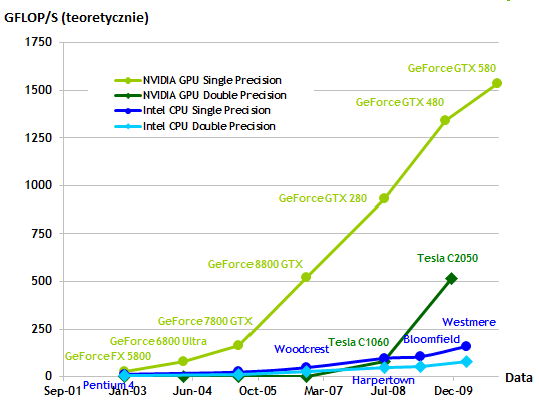
\includegraphics[width=0.9\textwidth]{figures/03/gpu_cpu2.png}
\caption{Operacje zmiennopozycyjne na sekundę na GPU oraz CPU~\cite{Cuda:PGuide}}\label{rys:gpu_cpu2}
\end{figure}

Powodem tak dużej rozbieżności w możliwościach przetwarzania równoległego (zauważalne na rysunku~\ref{rys:gpu_cpu2}) pomiędzy CPU a GPU jest fakt wysokiej specjalizacji na intensywne obliczenia w sposób równoległy (czyli to, co jest głównym składnikiem renderowania grafiki) - dlatego też w jednostkach kart grafiki więcej tranzystorów przeznaczonych jest do przetwarzania danych zamiast na cache danych oraz przepływ sterowania - schematycznie zilustrowane to zostało na rysunku~\ref{rys:gpu_cpu_trans}.

\begin{figure}[h]
\centering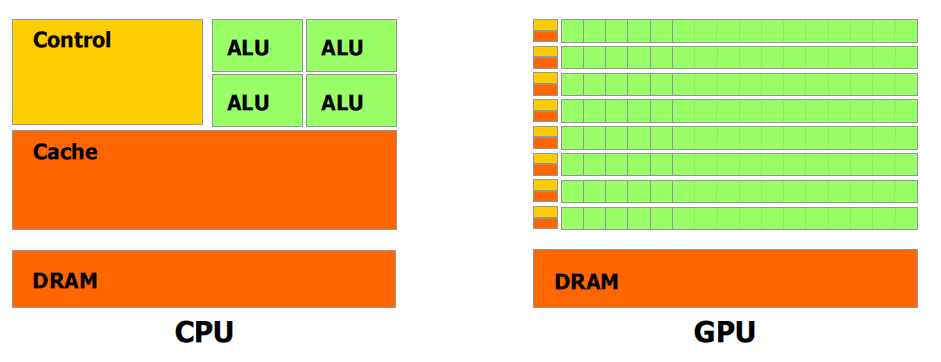
\includegraphics[width=1.0\textwidth]{figures/03/gpu_cpu_trans.png}
\caption{Schematyczne przedstawienie budowy CPU oraz GPU~\cite{Cuda:PGuide}}\label{rys:gpu_cpu_trans}
\end{figure}

Opisując bardziej szczegółowo, to GPU jest tak zaprojektowane by spełniać wymagania problemów, które mogą być zapisane jako obliczenia równoległę - ten sam program (metoda) jest wykonywany na każdym elemencie danych rónolegle. Ponieważ ten sam program jest uruchomiony na każdym elemencie danyh, to istnieje mniejsze wymaganie w kontroli skomplikowanego przepływu danych. Dodatkowo z powodu wysokiej intensywności arytmetycznej, to opóźnienie dostępu do pamięci może być ukryte przy pomocy obliczeń zamiast dużych części danych przechowywanych w cache jednostki.

Równoległe przetwarzanie danych mapuje elementy danych na równoległe wątki przetwarzające te dane. Wiele aplikacji, które przetwarzają duże zbiory danych może używać podejścia równoległego przetwarzania danych do przyspieszenia obliczeń. W renderowaniu grafiki 3D duże zbiory pikseli oraz wektory są mapowane na równoległe wątki. Podobnie w aplikacjach przetwarzających obraz oraz media, takie jak post-przetwarzanie wyrenderowanych obraów, kodowanie i  dekodowaniu video, skalowanie obrazó, czy też rozpoznawanie wzorców może mapować bloki obrazu oraz pikseli na równoległe wątki. W rzeczywistości, wiele algorytmów poza dziedziną przetwarzania obrazów są przyspieszane poprzez równoległe przetwarzanie danych - począwszy od przetwarzania sygnałów czy też symulacji fizycznych do obliczeń finansowych, czy też biologii oblieczniowej.

\subsection{Skalowalny model programistyczny}
Nadejście wielokorowych procesorów oraz multikorowych GPU oznacza, że główne chipy procesorowe są teraz systemami równoległymi. Co więcej równoległość kontynuuje skalowalność zgodnie z prawem Moora - czyli zgodnie z empirycznym prawem, które polega na obserwacji, że ekonomicznie optymalna liczba tranzystorów w układzie scalonym w kolejnych latach posiada trend wykładniczy (podwaja się w niemal równych odcinkach czasu). Wyzwaniem jest stworzenie takiego oprogramowanie, które w niezuważalny sposó będzie skalowało wykorzystywanie równoległości do zmieniającego się środowiska, w którym wzrastać będzie liczba korów procesora, zupełnie jak aplikacje graficzne, które transparentnie skalują swój paralelizm do wielu korów GPU, niezależnie od tego na jakiej karcie graficznej są one uruchamiane, co wiąże sie bezpośrednio z liczbą dostępnych jednostek na procesorze.

Równoległy model programistyczny CUDA jest stworzony by przezwyciężyć wyzwanie, o którym wspomniano wyżej, z jednoczesnym ograniczeniem czasu potrzebnego programistom na nauczenie się nowego podejścia poprzez wykorzystywanie do tworzenia aplikacji standardowych języków programowania, takich jak język C.

W swoim źródle CUDA posiada trzy kluczowe elementy: hierarchię grup wątków, współdzieloną pamięć oraz barierę synchronizacyjną. Elementy te są udostępnione programiście poprzez ograniczony zbiór rozszerzeń języka programowania.

Te abstrakcyjne elementy dostarczają drobnoziarnistą równoległość na poziomie danych oraz wątków, zagnieżdżone w gruboziarnistej równoległości danch oraz zadań (\english{task}). Takie podejście prowadzi programistę do podziału problemu na większe podproblemy, które mogą być rozwiązane niezależnie przez bloki wątków, a każdy podproblem może być podzielony na mniejsze, które mogą być rozwiązywane wspólnie przez wątki wewnątrz jednego bloku.

Taka dekompozycja zachowuje wszystkie dostępne funkcjonalności języka programowania umożliwiając wątkom kooperować w trakcie rozwiązywania każdego z podproblemów, a w tym samym czasie udostępnia automatyczną skalowalność programu. W rzeczywistości, każdy blok wątków może być zaplanowany na każdym z dostępnych korów na procesorze, w dowolnym porządku, jednocześnie lub sekwencyjnie, tak że skompilowany program w CUDA może być wykonany na dowolnej liczbnie korów procesora, jak zostało to zilustrowane na rysunku~\ref{rys:threads_gpu}. Jedynie \emph{system uruchomieniowy} (\english{runtime system}) musi znać faktyczną liczbę jednostek procesora. Wielowątkowy program jest podzielony na bloki wątkó, które wykonywane są niezależnie jeden od drugiego, dlatego też GPU z większą liczbą korów będzie automatycznie wykonywać program w krótszym czasie niż karta graficzna z mniejszą liczbą jednostek.

\begin{figure}[h]
\centering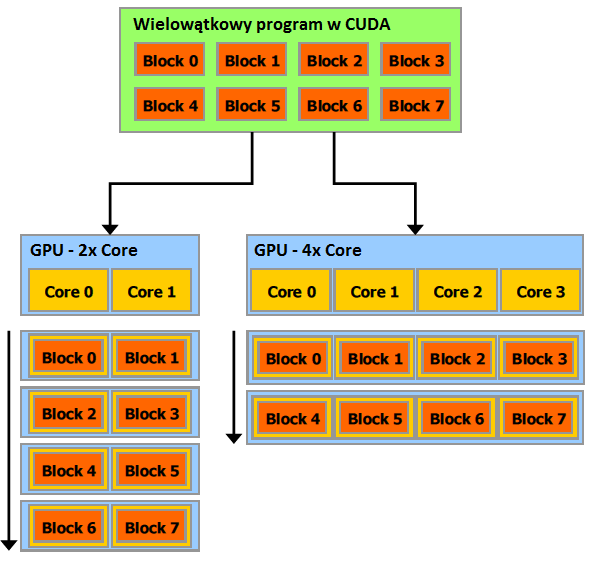
\includegraphics[width=1.0\textwidth]{figures/03/threads_gpu.png}
\caption{Zilustrowanie automatycznej skalowalności~\cite{Cuda:PGuide}}\label{rys:threads_gpu}
\end{figure}

Ten skalowalny model programistyczny umożliwia architekturze CUDA być stosowaną w szerokim spektrum zastosowań: od wysokowydajnych kart graficznych GeForce czy też na profesjonalnych kartach Quadro na komputerach entuzjastów, kartach Tesla przeznaczonych tylko do obliczeń, do kart GeForce przeznaczonych na domowe komputery.

\subsection{Używanie architektury CUDA}

Wysiłek wprowadzenia nowej architektury przez firmę NIDIA, która łączy możliwości klasycznego sposobu genercji grafiki z nowym podejściem do uniwersalnch obliczeń nie oznacza, że wprowadzono jedynie nową architekturę, bez odpowiedniego podejścia dla programowania. Bez względu na to, ile nowych funkcjonalności NVIDIA doda do swoich chipów, niemożliwe stało się używanie ich w dotychczasowy sposób - tj. poprzez OpenGL lub DirectX. Nie tylko wymagałoby to od użytkowników dalszego przekształcania swoich algorytmów do problemów renderowania grafiki (problem opisany w części~\ref{chapter:wczesne}), ale również w dalszym ciągu użytkownicy (programiści) musieli by programować swoje obliczenia w zorientowanych na renderowanie grafiki środowiskach (tzw. \emph{shading languages}) takich jak GLSL z OpenGL'a czy też HLSL firmy Microsoft.

By osiągnąć możliwie wysoki poziom developerów korzystających z możliwości nowej architektury, NVIDIA rozszeszyła jeden z najbardziej znanych języków programownia - język C, dodając do niego relatywnie mały zbiór nowych słów kluczowych, by programiści mogli korzystać z nowych, specjalnych funkcji dostępnych jedynie na architekturze CUDA. Kilka miesiecy po wprowadzeniu karty GeForce 8800 GTX~\cite{nvidia:geforce8800}, NVIDIA wprowadziła na rynek darmowy kompilator dla języka CUDA C~\cite{cuda:downloads}. W tym samym momencie, CUDA C stał się pierwszym językiem zaprojektowanym przez firmę produkującą sprzęt graficzny w celu wypełnienia luki w obliczeniach ogólnego przeznaczenia realizowanych na kartach graficznych.

Oprócz języka, w którym tworzone mogą być programy korzystające z mocy GPU, NVIDIA dostarczyła również specjalne \emph{sterowniki} (\english{drivers}) by wykorzystać pełną moc architektury CUDA. Użytkownicy nie są już więcej zobowiązani do znania interfejsów programowania specyficznych dla procesorów graficznych (takich jak OpenGL czy też DirectX), a co więcej nie są już oni zmuszeni do sprowadzanie swoich problemów do problemu renderowania grafiki.